\begin{figure}[h!]
	\centering
	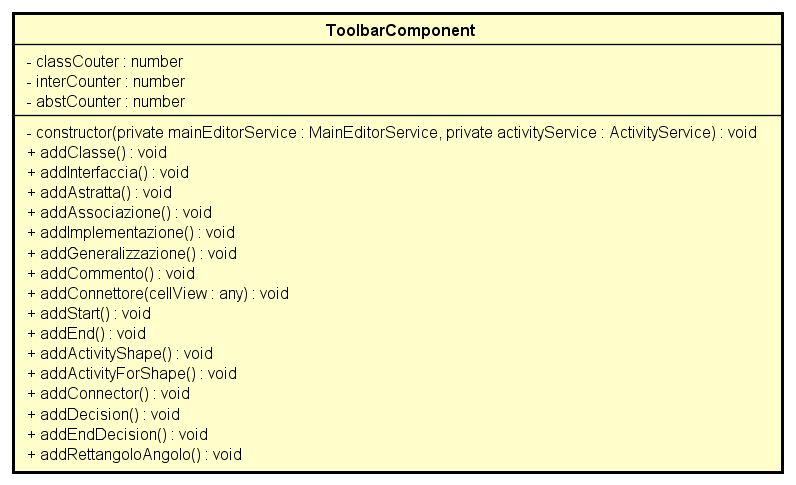
\includegraphics[scale=0.8]{res/sections/SpecificaFrontEnd/Components/Disegnetti/toolbar.png}
	\caption{Diagramma della classe ToolbarComponent}
\end{figure}

\begin{itemize}
	\item \textbf{Descrizione:}\\
	
	\item \textbf{Utilizzo:}\\
	
	\item \textbf{Attributi:}
		\begin{itemize}
			\item \emph{-classCouter: number}\\
			Conta il numero di classi presenti nell'editor
			\item \emph{-interCounter: number}\\
			Conta il numero di interfacce presenti nell'editor
			\item \emph{-abstCounter: number}\\
			Conta il numero di classi astratte presenti nell'editor
		\end{itemize}
	\item \textbf{Metodi:}
		\begin{itemize}
			\item \emph{-constructor(private mainEditorService: MainEditorService, private activityService: ActivityService)}\\
    		Costruttore della classe\\
    		\textbf{Parametri:}
    		\begin{itemize}
    			\item \emph{mainEditorService: MainEditorService}\\
    			Crea un istanziazione di MainEditorService
    			\item \emph{activityService: ActivityService}\\
    			Crea un istanziazione di AcrivityService
    		\end{itemize}
    		\item \emph{+addClasse()}\\
    		Aggiunge una classe all'editor
    		\item \emph{+addInterfaccia()}\\
    		Aggiunge un interfaccia all'editor
    		\item \emph{+addAstratta()}\\
    		Aggiunge una classe astratta all'editor
    		\item \emph{+addAssociazione()}\\
    		Seleziona il tipo di connettore \textit{Associazione}
    		\item \emph{+addImplementazione()}\\
    		Seleziona il tipo di connettore \textit{Implementazione}
    		\item \emph{+addGeneralizzazione()}\\
    		Seleziona il tipo di connettore \textit{Generalizzazione}
    		\item \emph{+addCommento()}\\
    		Aggiunge un commento all'editor
    		\item \emph{+addConnettore(cellView: any)}\\
    		Aggiunge il connettore selezionato
    			\begin{itemize}
    			\item \emph{cellView: any}\\
    			Elemento target o source
    		\end{itemize}
    		\item \emph{+addStart()}\\
    		Aggiunge l'elemento start all'editor
    		\item \emph{+addEnd()}\\
    		Aggiunge l'elemento end all'editor
    		\item \emph{+addActivityShape()}\\
    		Aggiunge un azione
    		\item \emph{+addConnector()}\\
    		Seleziona il connettore freccia per l'activity diagram
    		\item \emph{+addDecision()}\\
    		Aggiunge all'editor un inizio if/ciclo
    		\item \emph{+addEndDecision()}\\
    		Aggiunge all'editor una fine if/ciclo
    		\item \emph{+addRettangoloAngolo()}\\
    		Aggiunge un attività
		\end{itemize}
\end{itemize}